
\section{Numerical Methods}

\begin{frame}{Transition}

  Need a transition and overview for the numerics here.
  
\end{frame}

%\begin{frame}{It\^{o}'s Formulas}
\begin{frame}{Ito's Formulas}
  	\begin{itemize}
   		\item First version: $$f(B(b))-f(B(a))=\int_{a}^{b}{\frac{\partial f}{\partial B} 				dB}+\int_{a}^{b}{\frac{1}{2} \frac{\partial^2 f}{\partial B^2} dt} $$\\
    		\item Second version: $$f(b,B(b))-f(a,B(a))=\int_{a}^{b}{\frac{\partial f}{\partial B} 			dB}+\int_{a}^{b}{(\frac{\partial f}{\partial s}+\frac{1}{2}\frac{\partial ^2 f}{\partial 		B^2}) ds}$$\\
  		\item  Third version: The Stochastic Chain Rule $$d\theta=\frac{\partial\theta}{\partial 		t}dt+\frac{\partial\theta}{\partial x}f dB+\frac{\partial\theta}{\partial x}g 					dt+\frac{1}{2}\frac{\partial^2\theta}{\partial x^2}f^2dt$$
  	\end{itemize}
\end{frame}

\begin{frame}{Numerical methods}
Integral form of a SDE: 
$$X(t)=X_0+\int_{0}^{t}f(X(s))ds+\int_{0}^{t}g(X(s))dW(s)$$

X(t) is a random variable for each value of t. To apply numerical methods:
	\begin{itemize}
		\item Discretized time steps	
		\item X(t) will be the limit as our stepsize goes to cero.
	\end{itemize}
\end{frame}

\begin{frame}{Euler-Maruyama method}
Let $X_j=X(\tau_j)$ and $\tau_j=j\Delta t$. In the in the interval [0,L] we have:\bigskip\\
$$X_j=X_{j-1}+f(X_{j-1})\Delta t+g(X_{j-1})(W(\tau_j)-W(\tau_{j-1}))$$
 An approximation for:
$$X(\tau_j)=X(\tau_{j-1})+\int_{\tau_{j-1}}^{\tau_{j}}f(X(s))ds+\int_
{\tau_{j-1}}^{\tau_{j}}X(s))dW(s)$$
%We have Euler's method in the deterministic case ($g\equiv 0$)
\end{frame}

\begin{frame}
\begin{block}{Strong Convergence}
We say that a method has strong order of convergence equal to $\gamma$ if there exists a constant C such that:
$$E|X_n-X(\tau)|\leq C \Delta t^\gamma$$
for any fixed $\tau=n \Delta t \in [0,T]$ and $\Delta t$ sufficiently small.
\end{block}
\bigskip
The EM method has strong order of convergence of $\gamma=\frac{1}{2}$.
\end{frame}

\begin{frame}{Milstein's method}
To raise the strong order of convergence to 1:	

*I need something else here.

	\begin{equation*}
	\begin{split}
	X_{j} & =X_{j-1}+\Delta t f(X_{j-1})+g(X_{j-1})(W(\tau_j)-W(\tau_{j-1}))\\
	  &\quad +\frac{1}{2}g(X_{j-1})g'(X_{j-1})((W(\tau_j)-W(\tau_{j-1}))^2-\Delta t)
	\end{split}
	\end{equation*}
\end{frame}

\begin{frame}{Example}

  Discuss the example.
  
\end{frame}

\begin{frame}
	\begin{center}
	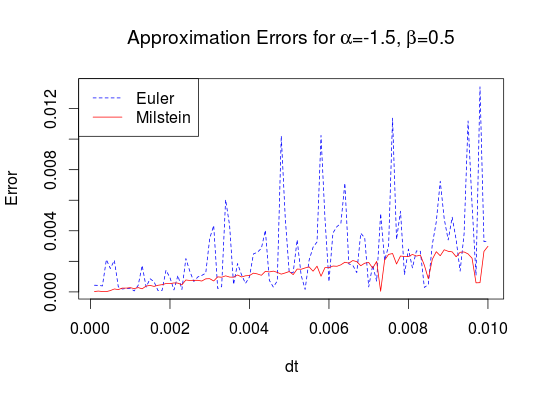
\includegraphics[scale=0.55]{alpham15_beta05.png} 
	\end{center}
\end{frame}

\begin{frame}
For systems of equations:
	\begin{eqnarray*}
		dx&=&f_1(x,y)dt+g_1(x,y)dW\\
		dy&=&f_2(x,y)dt+g_2(x,y)dW\\
	\end{eqnarray*}
In their integral form:
	\begin{eqnarray*}
		x_t=x_a+\int_{a}^{t}f_1 ds+\int_{a}^{t}g_1dW_1\\
		y_t=y_a+\int_{a}^{t}f_2 ds+\int_{a}^{t}g_2dW_2\\
	\end{eqnarray*}	
\end{frame}

\begin{frame}
If we apply the chain rule for $f_1$:
	\begin{equation*}
	\begin{split}
	f_1(\tau_j) &=f_1(\tau_{j-1})+f_{1x}(\tau_{j-1})(x-x(\tau_{j-1}))+f_{1y}(\tau_{j-1})(y-y(\tau_{j-1}))+\frac{1}{2} f_{1xx}(\tau_{j-1})(x-x(\tau_{j-1}))^2\\
		   &\quad +f_{1xy}(\tau_{j-1})(x-x(\tau_{j-1}))(y-y(\tau_{j-1}))+\frac{1}{2}f_{1yy}(\tau_{j-1})(y-y(\tau_{j-1}))^2
	\end{split}
	\end{equation*}
From the integral form:
	\begin{equation*}
	x(\tau_{j})-x(\tau_{j-1})=\int_{\tau_{j-1}}^{\tau_{j}}f_1 ds+\int_{\tau_{j-1}}^{\tau_{j}}g_1dW_1
	\end{equation*}

\end{frame}

\begin{frame}

%I need to fix how it looks
Similarly for $g_1$ and ignoring the high order terms:
	\begin{equation*}
	\begin{split}
	x(\tau_{j})&=x(\tau_{j-1})+f_1(\tau_{j-1})\Delta t+g_1(\tau_{j-1})\Delta W_1+\\
	&\quad g_{1x}(\tau_{j-1})\int_{\tau_{j-1}}^{\tau_{j}}\int_{\tau_{j-1}}^{s}g_1dW_1dW_1 +g_{1y}(\tau_{j-1})\int_{\tau_{j-1}}^{\tau_{j}}\int_{\tau_{j-1}}^{t} 		    g_2dW_2dW_1\\
	\end{split}
	\end{equation*}
Applying the chain rule again:
	\begin{equation*}
	\begin{split}
	x(\tau_{j})&=x(\tau_{j-1})+f_1(\tau_{j-1})\Delta t+g_1(\tau_{j-1})\Delta W_1\\
	&\quad +\frac{1}{2}g_{1x}(\tau_{j-1})g_{1}(\tau_{j-1})(\Delta W_1^2-\Delta t)\\
	&\quad +g_{1y}(\tau_{j-1})g_2(\tau_{j-1})\Delta W_1 \Delta W_2\\
	\end{split}
	\end{equation*}
\end{frame}

\begin{frame}
Similarly:
\begin{equation*}
	\begin{split}
	y(\tau_{j})&=y(\tau_{j-1})+f_2(\tau_{j-1})\Delta t+g_2(\tau_{j-1})(W_2(\tau_{j})-W_2(\tau_{j-1}))\\
	&\quad +\frac{1}{2}g_{2x}(\tau_{j-1})g_{1}(\tau_{j-1})(W_1(\tau_{j})-W_1(\tau_{j-1}))(W_2(\tau_{j})-W_2(\tau_{j-1}))\\
	&\quad +g_{2y}(\tau_{j-1})g_2(\tau_{j-1})((W_2(\tau_{j-1})-W_2(\tau_{j-1}))^2-\Delta t)\\
	\end{split}
	\end{equation*}
\end{frame}




